%% For double-blind review submission, w/o CCS and ACM Reference (max submission space)
\documentclass[sigplan]{acmart}\settopmatter{printfolios=true,printccs=false,printacmref=false}
\settopmatter{printacmref=false} % Removes citation information below abstract
\renewcommand\footnotetextcopyrightpermission[1]{} % removes footnote with conference information in first column
\pagestyle{plain} % removes running headers

%% For double-blind review submission, w/ CCS and ACM Reference
%\documentclass[acmsmall,review,anonymous]{acmart}\settopmatter{printfolios=true}
%% For single-blind review submission, w/o CCS and ACM Reference (max submission space)
%\documentclass[acmsmall,review]{acmart}\settopmatter{printfolios=true,printccs=false,printacmref=false}
%% For single-blind review submission, w/ CCS and ACM Reference
%\documentclass[acmsmall,review]{acmart}\settopmatter{printfolios=true}
%% For final camera-ready submission, w/ required CCS and ACM Reference
%\documentclass[acmsmall]{acmart}\settopmatter{}


%% Journal information
%% Supplied to authors by publisher for camera-ready submission;
%% use defaults for review submission.
\acmJournal{PACMPL}
\acmVolume{1}
\acmNumber{POPL} % CONF = POPL or ICFP or OOPSLA
\acmArticle{1}
\acmYear{2019}
\acmMonth{1}
\acmDOI{} % \acmDOI{10.1145/nnnnnnn.nnnnnnn}
\startPage{1}

%% Copyright information
%% Supplied to authors (based on authors' rights management selection;
%% see authors.acm.org) by publisher for camera-ready submission;
%% use 'none' for review submission.
\setcopyright{none}
%\setcopyright{acmcopyright}
%\setcopyright{acmlicensed}
%\setcopyright{rightsretained}
%\copyrightyear{2018}           %% If different from \acmYear

%% Bibliography style
\bibliographystyle{ACM-Reference-Format}
%% Citation style
%% Note: author/year citations are required for papers published as an
%% issue of PACMPL.
\citestyle{acmauthoryear}   %% For author/year citations


\usepackage{url}
\usepackage{amsmath}
\usepackage{amsfonts}
\usepackage{amssymb}
\usepackage{listings}
\usepackage{color}
\usepackage{graphicx}

%% https://github.com/nickgian/thesis/blob/master/lstcoq.sty
\usepackage{color}

\definecolor{ltblue}{rgb}{0,0.4,0.4}
\definecolor{dkblue}{rgb}{0,0.1,0.6}
\definecolor{dkgreen}{rgb}{0,0.35,0}
\definecolor{dkviolet}{rgb}{0.3,0,0.5}
\definecolor{dkred}{rgb}{0.5,0,0}

% lstlisting coq style (inspired from a file of Assia Mahboubi)
%
\lstdefinelanguage{Coq}{ 
%
% Anything betweeen $ becomes LaTeX math mode
mathescape=true,
%
% Comments may or not include Latex commands
texcl=false, 
%
% Vernacular commands
morekeywords=[1]{Section, Module, End, Require, Import, Export,
  Variable, Variables, Parameter, Parameters, Axiom, Hypothesis,
  Hypotheses, Notation, Local, Tactic, Reserved, Scope, Open, Close,
  Bind, Delimit, Definition, Let, Ltac, Fixpoint, CoFixpoint, Add,
  Morphism, Relation, Implicit, Arguments, Unset, Contextual,
  Strict, Prenex, Implicits, Inductive, CoInductive, Record,
  Structure, Canonical, Coercion, Context, Class, Global, Instance,
  Program, Infix, Theorem, Lemma, Corollary, Proposition, Fact,
  Remark, Example, Proof, Goal, Save, Qed, Defined, Hint, Resolve,
  Rewrite, View, Search, Show, Print, Printing, All, Eval, Check,
  Projections, inside, outside, Def, Polymorphic},
%
% Gallina
morekeywords=[2]{forall, exists, exists2, fun, fix, cofix, struct,
  match, with, end, as, in, return, let, if, is, then, else, for, of,
  nosimpl, when},
%
% Sorts
morekeywords=[3]{Type, Prop, Set, true, false, option},
%
% Various tactics, some are std Coq subsumed by ssr, for the manual purpose
morekeywords=[4]{pose, set, move, case, elim, apply, clear, hnf,
  intro, intros, generalize, rename, pattern, after, destruct,
  induction, using, refine, inversion, injection, rewrite, setoid_rewrite, congr,
  unlock, compute, ring, field, fourier, replace, setoid_replace, fold, unfold,
  change, cutrewrite, simpl, have, suff, wlog, suffices, without,
  loss, nat_norm, assert, cut, trivial, revert, bool_congr, nat_congr,
  symmetry, transitivity, auto, split, left, right, autorewrite},
%
% Terminators
morekeywords=[5]{by, done, exact, reflexivity, tauto, romega, omega,
  assumption, solve, contradiction, discriminate},
%
% Control
morekeywords=[6]{do, last, first, try, idtac, repeat},
%
% Comments delimiters, we do turn this off for the manual
morecomment=[s]{(*}{*)},
%
% Spaces are not displayed as a special character
showstringspaces=false,
%
% String delimiters
morestring=[b]",
morestring=[d]’,
%
% Size of tabulations
tabsize=3,
%
% Enables ASCII chars 128 to 255
extendedchars=false,
%
% Case sensitivity
sensitive=true,
%
% Automatic breaking of long lines
breaklines=false,
%
% Default style fors listings
basicstyle=\small,
%
% Position of captions is bottom
captionpos=b,
%
% flexible columns
basewidth={2em, 0.5em},
columns=flexible,
%
% Style for (listings') identifiers
identifierstyle={\ttfamily\color{black}},
% Style for declaration keywords
keywordstyle=[1]{\ttfamily\bfseries\color{dkviolet}},
% Style for gallina keywords
keywordstyle=[2]{\ttfamily\bfseries\color{dkgreen}},
% Style for sorts keywords
keywordstyle=[3]{\ttfamily\bfseries\color{ltblue}},
% Style for tactics keywords
keywordstyle=[4]{\ttfamily\color{dkblue}},
% Style for terminators keywords
keywordstyle=[5]{\ttfamily\color{dkred}},
%Style for iterators
%keywordstyle=[6]{\ttfamily\color{dkpink}},
% Style for strings
stringstyle=\ttfamily,
% Style for comments
commentstyle={\ttfamily\itshape\color{dkgreen}},
%
%moredelim=**[is][\ttfamily\color{red}]{/&}{&/},
literate=
    {fun}{{\color{dkgreen}{$\lambda\;$}}}1
    {bool}{{$\mathbb{B}$}}1
    {nat}{{$\mathbb{N}$}}1
    {Vforall2}{Vforall2}1 % quick workardoun to avoid partial replacement of 'forall' in identifier
    {nat\_equiv}{nat\_equiv}1 % quick workardoun to avoid partial replacement of 'nat' in identifier
    {forall}{{\color{dkgreen}{$\forall\;$}}}1
    {exists}{{$\exists\;$}}1
    {<-}{{$\leftarrow\;\;$}}1
    {=>}{{$\Rightarrow\;\;$}}1
    {==}{{\texttt{==}\;}}1
    {==>}{{$\Longrightarrow\;\;$}}1
%    {:>}{{\texttt{:>}\;}}1
    {->}{{$\rightarrow\;\;$}}1
    {<-->}{{$\longleftrightarrow\;\;$}}1
    {<->}{{$\leftrightarrow\;\;$}}1
    {<==}{{$\leq\;\;$}}1
    {\#}{{$^\star$}}1 
    {\\o}{{$\circ\;$}}1 
%    {\@}{{$\cdot$}}1 
    {\/\\}{{$\wedge\;$}}1
    {\\\/}{{$\vee\;$}}1
    {++}{{\texttt{++}}}1
    {~}{{\ }}1
    {¬}{{$\lnot$}}1     % this does not work
    {\@\@}{{$@$}}1
    {\\mapsto}{{$\mapsto\;$}}1
    {\\hline}{{\rule{\linewidth}{0.5pt}}}1
%
}[keywords,comments,strings]

\lstnewenvironment{coq}{\lstset{language=Coq}}{}

% pour inliner dans le texte
\def\coqe{\lstinline[language=Coq, basicstyle=\small]}
% pour inliner dans les tableaux / displaymath...
\def\coqes{\lstinline[language=Coq, basicstyle=\scriptsize]}

%%% Local Variables: 
%%% mode: latex
%%% Local IspellDict: british
%%% TeX-master: "main.tex"
%%% End: 
%\usepackage{booktabs}   %% For formal tables:
%\usepackage{subcaption}

\newcommand{\N}{\mathbb{N}}

\begin{document}

%% Title information
\title{Reification of shallow-embedded DSLs in Coq with automated verification}         %% [Short Title] is optional;
                                        %% when present, will be used in
                                        %% header instead of Full Title.
%\titlenote{with title note}             %% \titlenote is optional;
                                        %% can be repeated if necessary;
                                        %% contents suppressed with 'anonymous'
%\subtitle{Subtitle}                     %% \subtitle is optional
%\subtitlenote{with subtitle note}       %% \subtitlenote is optional;
                                        %% can be repeated if necessary;
                                        %% contents suppressed with 'anonymous'


\author{Vadim Zaliva}
\affiliation{
  \institution{Carnegie Mellon University}
}
\email{vzaliva@cmu.edu}

\author{Matthieu Sozeau}
\affiliation{
  \institution{Inria \& IRIF, University Paris 7}
}
\email{matthieu.sozeau@inria.fr}


\begin{abstract}
  Shallow and deep embeddings of DSLs have their pros and cons. For example,
  shallow embeddings are excellent for quick prototyping, as it allows
  quick extension or modification of the embedded language.  Meanwhile, deep
  embeddings are better suited for code transformation and compilation.
  Thus, it might be useful to be able to switch from shallow to deep
  embedding while making sure the semantics of the embedded language are
  preserved. We will demonstrate a working approach for implementing
  and proving such conversion using TemplateCoq.
\end{abstract}


%% 2012 ACM Computing Classification System (CSS) concepts
%% Generate at 'http://dl.acm.org/ccs/ccs.cfm'.
%\begin{CCSXML}
%<ccs2012>
%<concept>
%<concept_id>10011007.10011006.10011008</concept_id>
%<concept_desc>Software and its engineering~General programming languages</concept_desc>
%<concept_significance>500</concept_significance>
%</concept>
%<concept>
%<concept_id>10003456.10003457.10003521.10003525</concept_id>
%<concept_desc>Social and professional topics~History of programming languages</concept_desc>
%<concept_significance>300</concept_significance>
%</concept>
%</ccs2012>
%\end{CCSXML}

%\ccsdesc[500]{Software and its engineering~General programming languages}
%\ccsdesc[300]{Social and professional topics~History of programming languages}
%% End of generated code


%% Keywords
%% comma separated list
%\keywords{coq}  %% \keywords are mandatory in final camera-ready submission


%% \maketitle
%% Note: \maketitle command must come after title commands, author
%% commands, abstract environment, Computing Classification System
%% environment and commands, and keywords command.
\maketitle

\section{Introduction}

In the course of our work on the HELIX system \cite{helixFHPC18}, we faced
the problem of writing a certified compiler for a domain specific
language called $\Sigma$-HCOL, which is shallow-embedded in the Gallina
language of the Coq proof assistant \cite{Coq}. The approach presented in
this report is the result of a summer of 2018 collaborative visit to Inria,
where the use of TemplateCoq \cite{anand2018towards} was first suggested by
Matthieu Sozeau and successfully implemented and used in the HELIX
project.

An application of this technique to reify $\Sigma$-HCOL can be found
in the HELIX source code. For illustrative purposes in this paper, we use a simpler language of arithmetic expressions on natural
numbers. It is shallow-embedded in Gallina and includes constants,
bound variables, and three arithmetic operators: $+$, $-$, and
$*$, the complete source for which can be found in the git repository
\url{https://github.com/vzaliva/CoqPL19-paper}.

\subsection{Example}

Provided that $a, b, c, x \in \N$, the expression below is an example of a valid
expression in the source language:

\begin{lstlisting}[language=Coq, mathescape=true,
  basicstyle=\footnotesize,
  caption=Expression in source language,
  label=lst:sexp]
            2 + a*x*x + b*x + c.
\end{lstlisting}

The target language includes the same operators but will be defined by
an inductive type of its AST:

\begin{lstlisting}[language=Coq, mathescape=true,
  caption=Target language type,
  basicstyle=\footnotesize]
Inductive NExpr: Type :=
| NVar  : nat -> NExpr (* using Bruijn indices *)
| NConst: nat -> NExpr
| NPlus : NExpr -> NExpr -> NExpr
| NMinus: NExpr -> NExpr -> NExpr
| NMult : NExpr -> NExpr -> NExpr.
\end{lstlisting}

The expression from Listing~\ref{lst:sexp}, translated to the target
language, looks like:

\begin{lstlisting}[language=Coq, mathescape=true,
  basicstyle=\footnotesize,
  caption=Expression in target language, label=lst:texp]
NPlus (NPlus (NPlus (NConst 2)
  (NMult (NMult (NVar 3) (NVar 0)) (NVar 0)))
    (NMult (NVar 2) (NVar 0))) (NVar 1)
\end{lstlisting}

The purpose of the reification step is just to switch from shallow to
deep embedding. Thus, the target language syntax is supposed to be close
to the source language syntax. We just change the representation and
enforce the scope of the shallow embedding to ensure that only the
allowed subset of Gallina is used. This makes the translation
implementation fairly straightforward. Additionally, this allows
automatic proof of semantic preservation as shown below.

\section{Translation}

The translation process performs reification of a given expression,
producing a translated expression in the target language. It is implemented as a
\textit{template program} named \emph{reifyNExp}.

The input expressions are presented in a closed form, where all
variables first need to be introduced via lambda bindings. Thus, the
input expression could be either just $\N$ in the simplest case or
an n-ary function of natural numbers, for example $\N \rightarrow \N \rightarrow \N$.
The reification template program is hence polymorphic on the input type
expression.

In addition to the input expression, \emph{reifyNExp} takes two names
(as strings). The first is used as the name of a new
definition, to which the expression in the target language will be
bound. The second is the name to which the semantic preservation lemma will be bound, as
discussed in the next section.

\begin{lstlisting}[language=Coq, mathescape=true,
  basicstyle=\footnotesize, caption=Reification program]
Polymorphic Definition reifyNExp@{t u}
  {A:Type@{t}} (res_name lemma_name: string) (nexpr:A)
  : TemplateMonad@{t u} unit.
\end{lstlisting}

When executed, if successful, \emph{reifyNExp} will create a new
definition and new lemma with the given names. If not, it will fail with
an error. The reason for a failure might that the expression contains
constructs which are legal in Gallina but not part of our embedded
language. The translation is implemented in a straightforward way,
traversing the Gallina AST of the original expression that Template-Coq
quoting produces.

\section{Semantics Preservation}

The semantic of our source language is defined by Gallina. On the other
hand, the inductive type representing the target language needs to be
given its own semantics. We do this by providing an evaluation function
for the deeply embededd terms. It takes an \textit{evaluation context}
which holds the current values of free variables, the expression being
evaluated, and returns the result as a natural number or \emph{None} in
case of error.

\begin{lstlisting}[language=Coq, mathescape=true,
  basicstyle=\footnotesize]
Definition evalContext:Type := list nat.
Fixpoint evalNexp ($\Gamma$:evalContext) (e:NExpr): option nat.
\end{lstlisting}

The evaluation may fail, for example, if the expression references a
variable not present in the evaluation context. As variables are
represented by their indices in $\Gamma$, this will happen if an index is greater
or equal to the length of $\Gamma$.

The semantic preservation is expressed as a heterogeneous relation
between expressions in the source and target languages:

\begin{lstlisting}[language=Coq, mathescape=true,
  basicstyle=\footnotesize]
Definition NExpr_term_equiv ($\Gamma$: evalContext)
  (d: NExpr) (s: nat) : Prop := evalNexp $\Gamma$ d = Some s.
\end{lstlisting}

Consequently, the lemma generated by \emph{reifyNExp} for our example in Listing~\ref{lst:sexp} 
will state semantic equivalence between its expression and that of Listing~\ref{lst:texp}:

\begin{lstlisting}[language=Coq, mathescape=true,
  basicstyle=\footnotesize]
forall x c b a : nat, NExpr_term_equiv [x; c; b; a]
    NPlus (NPlus (NPlus (NConst 2)
        (NMult (NMult (NVar 3) (NVar 0)) (NVar 0)))
        (NMult (NVar 2) (NVar 0))) (NVar 1)
    (2 + a * x * x + b * x + c)
\end{lstlisting}

The generated lemma still needs to be proven. Because the expressions
in the original and target languages have the same structure, such proof
can be automated. The general idea is to define and prove semantic
equivalence lemmas for each pair of operators and then add them as
hints into a hint database used with the \emph{eauto} tactic:

\begin{lstlisting}[language=Coq, mathescape=true,
  basicstyle=\footnotesize]
Lemma NExpr_add_equiv ($\Gamma$: evalContext) {a b a' b' }:
  NExpr_term_equiv $\Gamma$ a a' -> NExpr_term_equiv $\Gamma$ b b' ->
  NExpr_term_equiv $\Gamma$ (NPlus a b) (Nat.add a' b').

Lemma NExpr_mul_equiv ($\Gamma$: evalContext) {a b a' b' }:
  NExpr_term_equiv $\Gamma$ a a' -> NExpr_term_equiv $\Gamma$ b b' ->
  NExpr_term_equiv $\Gamma$ (NMult a b) (Nat.mul a' b').

Lemma NExpr_const_equiv ($\Gamma$: evalContext) {v v' }:
  evalNexp $\Gamma$ (NConst v) = Some v' ->
  NExpr_term_equiv $\Gamma$ (NConst v) v'.

Lemma NExpr_var_equiv ($\Gamma$: evalContext) {v x}:
  evalNexp $\Gamma$ (NVar v) = Some x ->
  NExpr_term_equiv $\Gamma$ (NVar v) x.

Create HintDb NExprHints.
Hint Resolve NExpr_add_equiv NExpr_mul_equiv: NExprHints.
Hint Resolve NExpr_const_equiv NExpr_var_equiv: NExprHints.

Obligation Tactic := intros; simpl; eauto 99 with NExprHints.
Run TemplateProgram (reifyNExp "Ex1_def" "Ex1_lemma" Ex1).
\end{lstlisting}

The ASTs of the original and translated expressions and the semantic
equivalence relations between them are shown in Figure~\ref{fig:trees}.

\begin{figure}[h]
  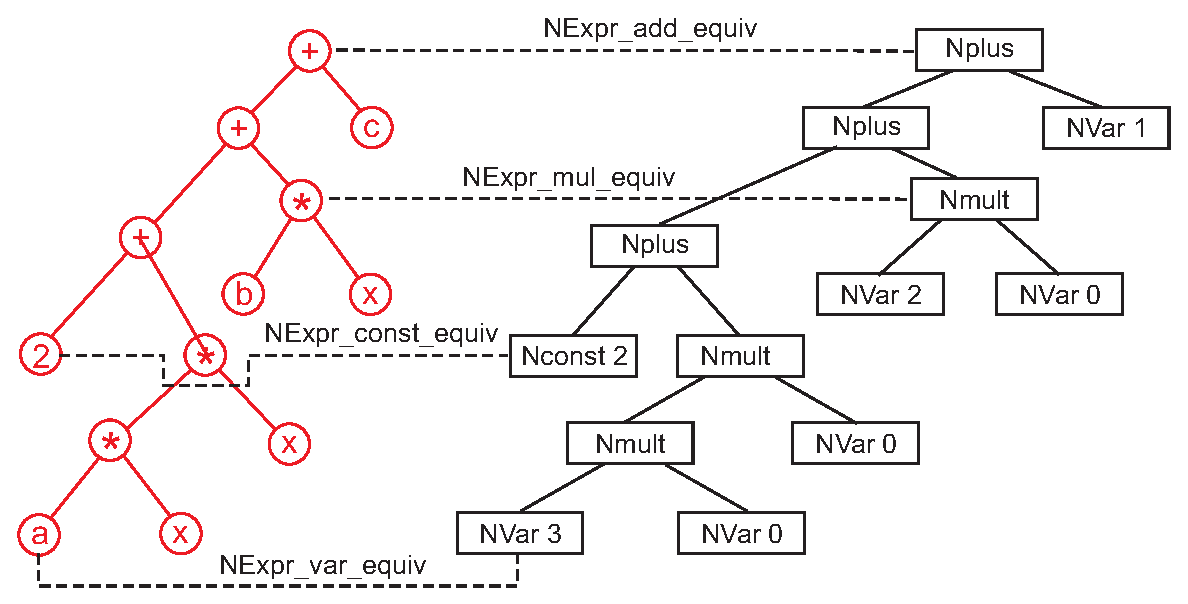
\includegraphics[width=\columnwidth]{trees.eps}
  \caption{Semantics equivalence}
  \label{fig:trees}
\end{figure}

\section{Summary}

Our approach could be summarized as follows. In order to translate a
language shallowly embedded in Gallina into a deep embedding, complete
the following steps:

\begin{enumerate}
\item Define an inductive type for the target language AST.
\item Implement an evaluation function for the target language.
\item Define a semantic equivalence relation between expressions in
  source and target languages.
\item Implement reification as a template program which generates an
  expression in the target language and a semantic preservation lemma.
\item Define and prove lemmas of semantic equivalence between
  operators of source and target languages and add them to the
  hints database.
\item Use \emph{eauto} to prove automatically generated semantic
  preservation lemma.  
\end{enumerate}

We successfully applied this translation validation approach to the
non-trivial $\Sigma$-HCOL language in HELIX, featuring binders,
dependent types, and higher-order operators like map on fixed-sized
vectors. We found it easy to implement compared to other means of
reification like type classes or LTac programming and recommend using
it as a guide for switching from shallow to deep embedding of DSLs. In
the presentation, we propose to present this case study in detail.

\nocite{*}
\bibliography{paper}

\end{document}

